%Note di Ingegneria del Software
%Sommario: Misurazioni Software

\cornell{Misurazione: Motivazioni e rischi}{Perchè?
\begin{itemize}
\item Per conoscere e imparare
\item Per valutare
\end{itemize}
Rischi connessi: Semplificazioni ed imprecisioni nelle misurazione possono provocare danni, anche gravi\\
La misura deve essere \textbf{oggettiva}, il che implica le seguenti caratteristiche: \begin{itemize}
\item Ripetibilità
\item Confrontabilità
\item Confidenza (posso fidarmi della misurazione)
\end{itemize}}

\cornell{Misurazione: Definizione}{Processo che assegna valori ad attributi di entità per descriverle secondo delle \textit{regole definite}}

\cornell{Misura}{\begin{itemize}
\item Il risultato della misurazione
\item Assegnazione di un valore quantitativo ad un'entità, per caratterizzarne un attributo specifico.
\end{itemize}}

\cornell{Metrica}{L'insieme di regole definite usate per la misurazione.}

\cornell{Indicatore}{Misura sintetica usata per caratteristiche o fenomeni non misurabili direttamente.\\
Tramite gli indicatori (misurabili) posso ricondurmi ad una misura della realtà che non è direttamente misurabile.}

\cornell{Come si forma una valutazione}{\begin{description}
\item[Serie Storiche] (Tendenze nel tempo)\\ Posso popolare una serie storica quando i valori cambiano (altrimenti non avrebbe senso).\\Per esempio per la serie storica riguardante delle lauree il popolamento potrebbe avvenire ogni anno
\item[Benchmark]\\Confronto con valori di riferimento derivanti dalle best practice (o best performance) del dominio\\Quindi si va a puntare verso un obiettivo o riferimento (solitamente autorevole)
\item[Adesione] ad una checklist di regole od obiettivi definiti
\end{description}}

\cornell{Obiettivi di Misurazione}{ \begin{description}
\item [Valutare lo stato di]\ \begin{itemize}
\item Progetti (Stime, preventivi/consuntivi di tempi/costi)
\item Prodotti (Misurando l'efficacia)
\item Processi (Misurando la capability/maturity ed eventuali miglioramenti)
\item Risorse (Misurando l'efficienza)
\end{itemize}
\item[Tramite Attributi]\ \begin{itemize}
\item Interni: Che misurano l'azione/fenomeno in sé
\item Esterni: che misurano il loro effetto o impatto
\end{itemize}
\item[Per interpretare/cogliere tendenze] In modo proattivo (invece di reattivo)
\item[Per intraprendere azioni correttive] Privilegiando quelle che danno maggior effetto col minor costo
\end{description}}

\cornell[Definizione Importante]{Modello}{Descrizione/Spiegazione della realtà, cioè spieghiamo il "perché" di una certa realtà}

\cornell{Processi di Misurazione}{ISO/IEC 15939 - Software Measurement Process\\
Suddiviso in: \begin{itemize}
\item \textbf{Measurement Information Model}\\Cosa misuriamo
\item \textbf{Measurement Process Model}\\Come lo misuriamo
\end{itemize}\\
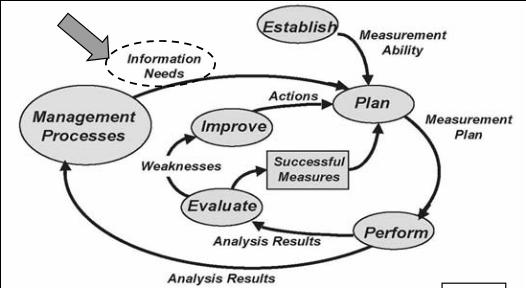
\includegraphics[scale=0.5]{images/73.png}}

\cornell{Information Needs}{Sono basati su obiettivi, limiti imposti, rischi e problemi che si originano da processi tecnici e di gestione}

\cornell{Esempi di information needs}{Per il management: \begin{itemize}
\item Costo di un Processo
\item Produttività degli sviluppatori
\item Qualità del prodotto
\end{itemize}\\
Per gli sviluppatori: \begin{itemize}
\item Verificabilità dei requisiti
\item Copertura dei requisiti
\item Quantità di difetti residui
\end{itemize}}

\cornell{Esempio: Modello di produttività}{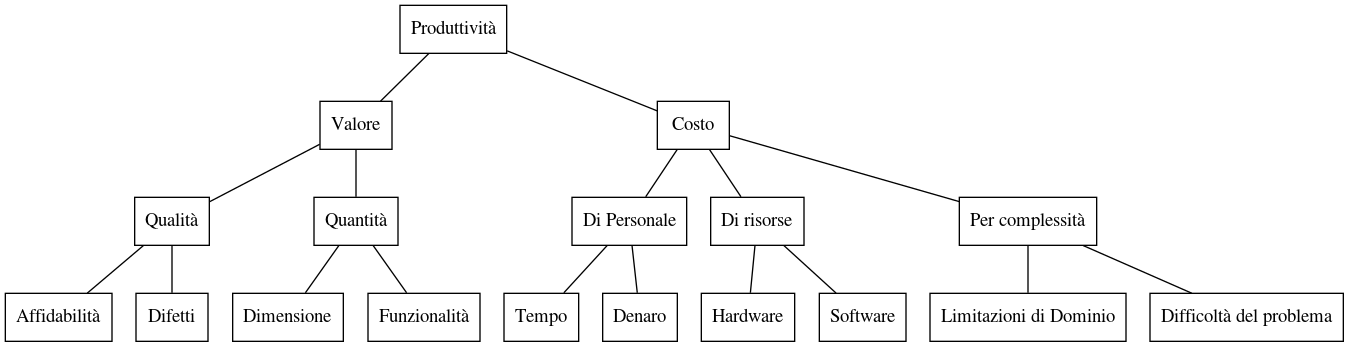
\includegraphics[scale=0.23]{images/74.png}}

\cornell{Lead Time}{Tempo (di calendario) tra l'apertura (assegnazione "alla comunità") di un ticket e la sua chiusura con successo (in cui l'obiettivo è raggiunto).\\
È una metrica di gestione del progetto}

\cornell{Metriche Software}{Problemi: \begin{itemize}
\item Il software è immateriale ed è quindi difficile da misurare
\item Il Software ha caratteristiche multiformi
\end{itemize}}

\cornell{Metriche di Progetto}{ \begin{itemize}
\item Grado di Coesione
\item Grado di Accoppiamento
\item Complessità Strutturale (Funzione del Fan-out)
\item Complessità del flusso dati (Funzione del numero di parametri in ingresso ed uscita, oltre alla complessità strutturale)
\item Complessità del sistema (Funzione della complessità strutturale e del flusso dati)
\end{itemize}}

\cornell{Metriche di Programmazione}{ \begin{itemize}
\item SLOC (Source Line of Code)
\item Conteggio di costrutti/comandi
\end{itemize}}

\cornell{Complessità Ciclomatica}{Complessità del flusso di controllo in funzione dei possibili cammini indipendenti all'interno di un singolo sottoprogramma.\begin{itemize}
\item 1-10 Bassa
\item 21-50 Alta
\item $>$50 Inaccettabile
\end{itemize}}

\cornell{Fallibilità della complessità ciclomatica}{Problemi rilevabili: \begin{itemize}
\item Errore in difetto\\In caso di codice molto offuscato, si potrebbe avere una complessità ciclomatica bassa, ma il codice potrebbe risultare poco comprensibile.
\item Errore in eccesso\\Ad esempio nel caso dello statement "switch", che viene conteggiato come una serie di if/elseif annidati, mentre invece risulta molto più leggibile di quest'ultimo.
\end{itemize}}

\cornell{Legame con la manutenzione}{Nonostante la metrica sia fallibile, empiricamente è stato dimostrato che i programmi con complessità ciclomatica alta hanno problemi di manutenzione.\\
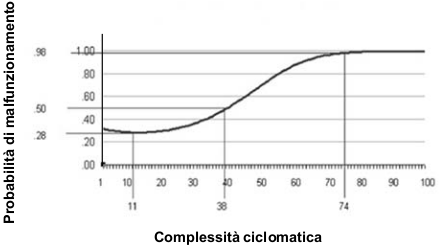
\includegraphics[scale=0.5]{images/75.png}}
